\section{Análise}
Todas as analises foram feitas baseadas em calculo de erro simples e utilizando o algoritmo de validação cruzada com 5 partições. Nestas análises não foram variadas o número de partições por acreditar que este trabalho prático é voltado para o algoritmo de \emph{boosting} e não de validação cruzada. Em todos os gráficos a seguir, o erro apresentando é a dado como a media do erro encontrado em cada validação cruzada.


A primeira análise interessante a ser feita é a relação dos errors tanto de treino quanto de validação com o número de iterações do \emph{Aadaboost}. Lembrando que o número de iterações é o número de classificadores fracos que queremos utilizar.

\begin{figure}[h]
  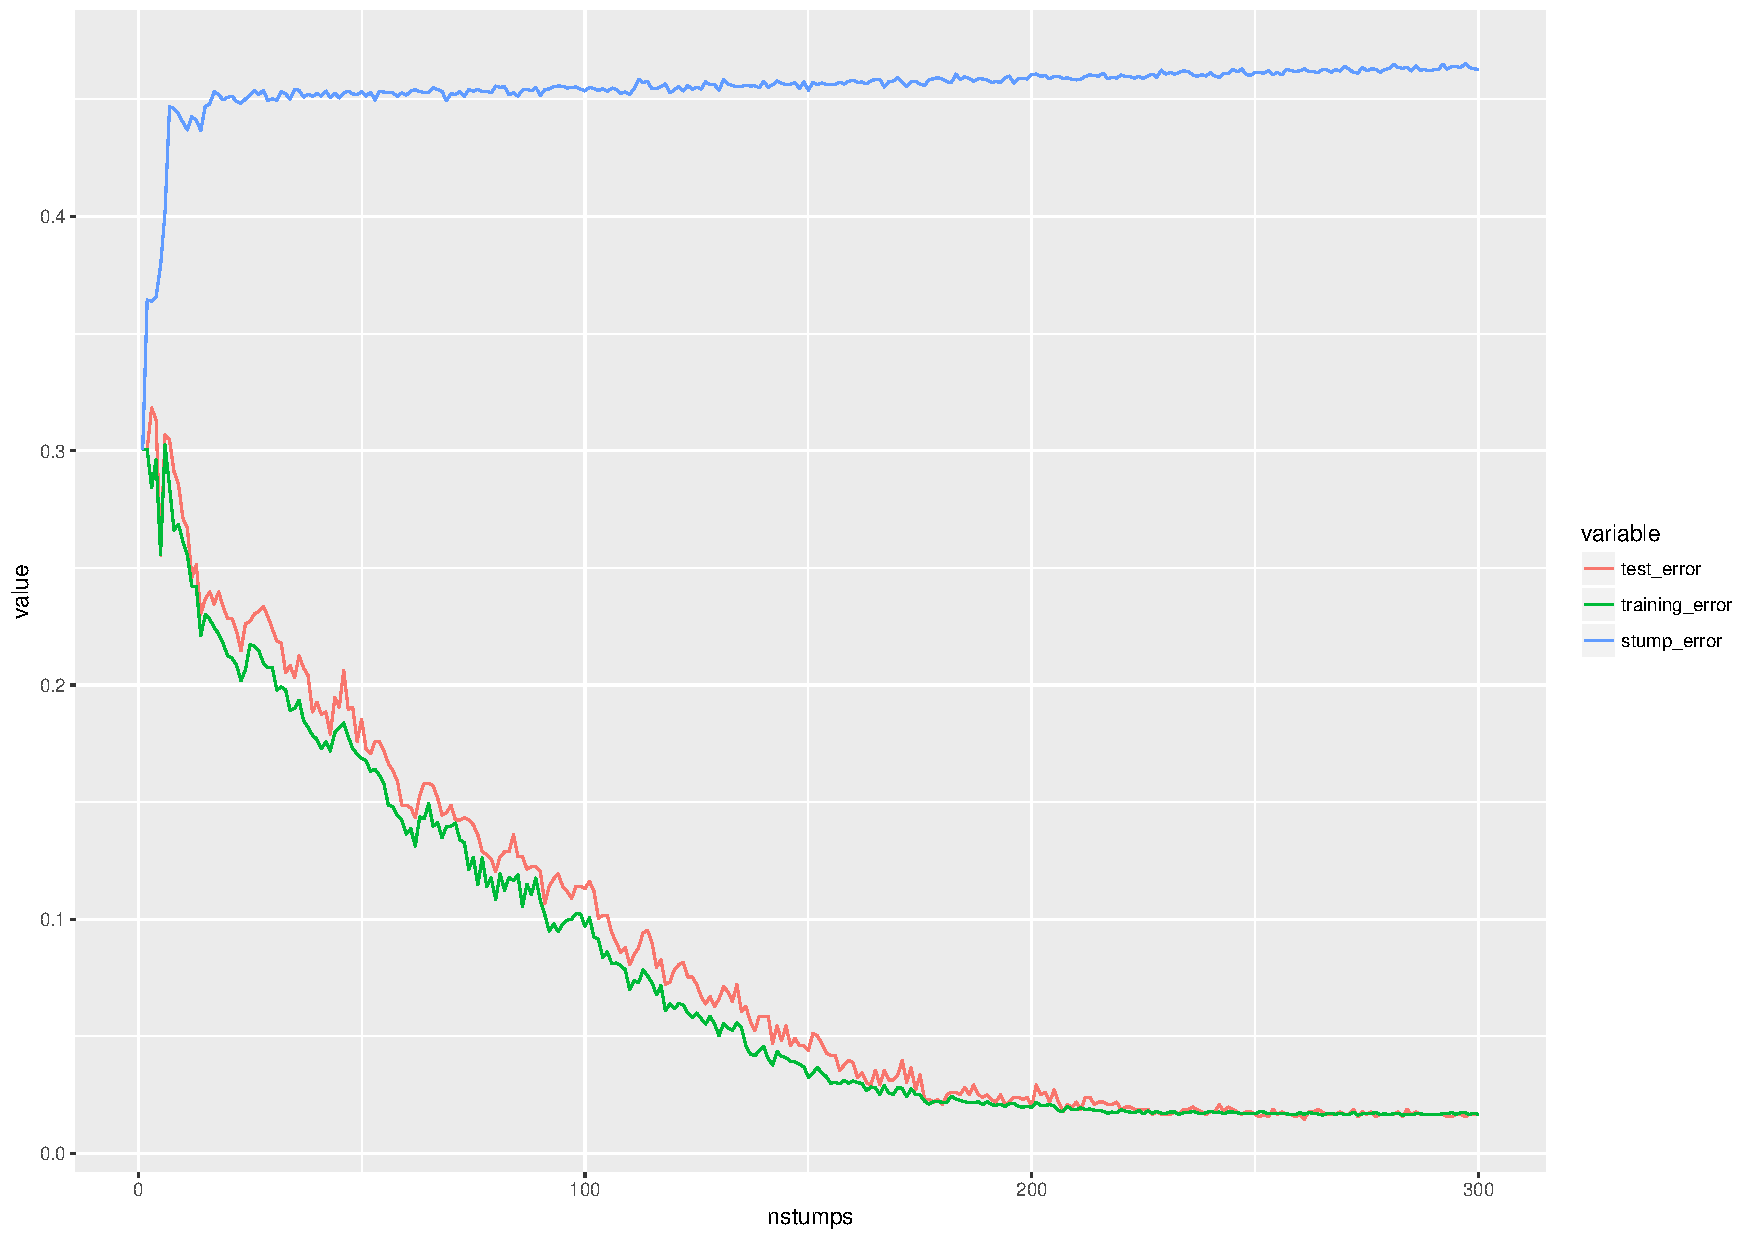
\includegraphics[width=\linewidth]{imgs/accuracy.pdf}
  \caption{Adaboost erros por quantidade de \emph{weak classifiers}}
  \label{fig:adaboostAccuracy}
\end{figure}

Como pode ser visto na Figura.~\ref{fig:adaboostAccuracy}, como esperado os errors de treino e de teste tendem a cair com o aumento de stumps escolhidos. Demonstrando assim a força da combinação de classificadores fracos, podemos ver que ambos convergem para um valor próximo de 0.02 tendo o erro de validação maior que o erro de treino durante a convergência. É interessante realçar que mesmo com uma grande escolha de um número grande de stumps, cerca de 6 vezes mais do que os stumps disponíveis, o \emph{Adaboost} não sofreu de \emph{overfit} e convergiu.

Outra padrão esperado que foi mostrado neste gráfico é o aumento do erro de cada stump escolhido (em cada uma das iterações) e sua convergência para um valor próximo de 0.5, mostrando assim, que idealmente, classificadores interessantes para o \emph{Adaboost} são aqueles um pouco melhores que o aleatório (0.5). 

Podemos ver também, que o primeiro stump escolhido já e responsável por aproximadamente 0.7 de acurácia (erro de 0.3 quando todas as observações tem a mesma importância), isso provavelmente deve ser fruto do desbalanceamento de classes, quase o dobro de partidas no dataset foram vencidas pelo jogador "x" (Tabela~\ref{tab:dataset}). Se olharmos com mais detalhes as Figuras~[\ref{fig:main2_2},\ref{fig:main_2_5}] veremos que o primeiro stump escolhido é o de identificação 27, que se consultarmos a Tabela~\ref{tab:stumps}, vemos que é o caso quando o jogador 'o' marcou na posição central do jogo da velha. O que faz sentido se pensarmos na estratégia ótima do jogo da velha. Este jogo é conhecido por ser desbalanceado de modo que quem começa se adotar a estratégia ótima não poderá perder, Se entrar em detalhes, tal estratégia envolve nunca preencher o quadrado central. 

\begin{figure}[h]
  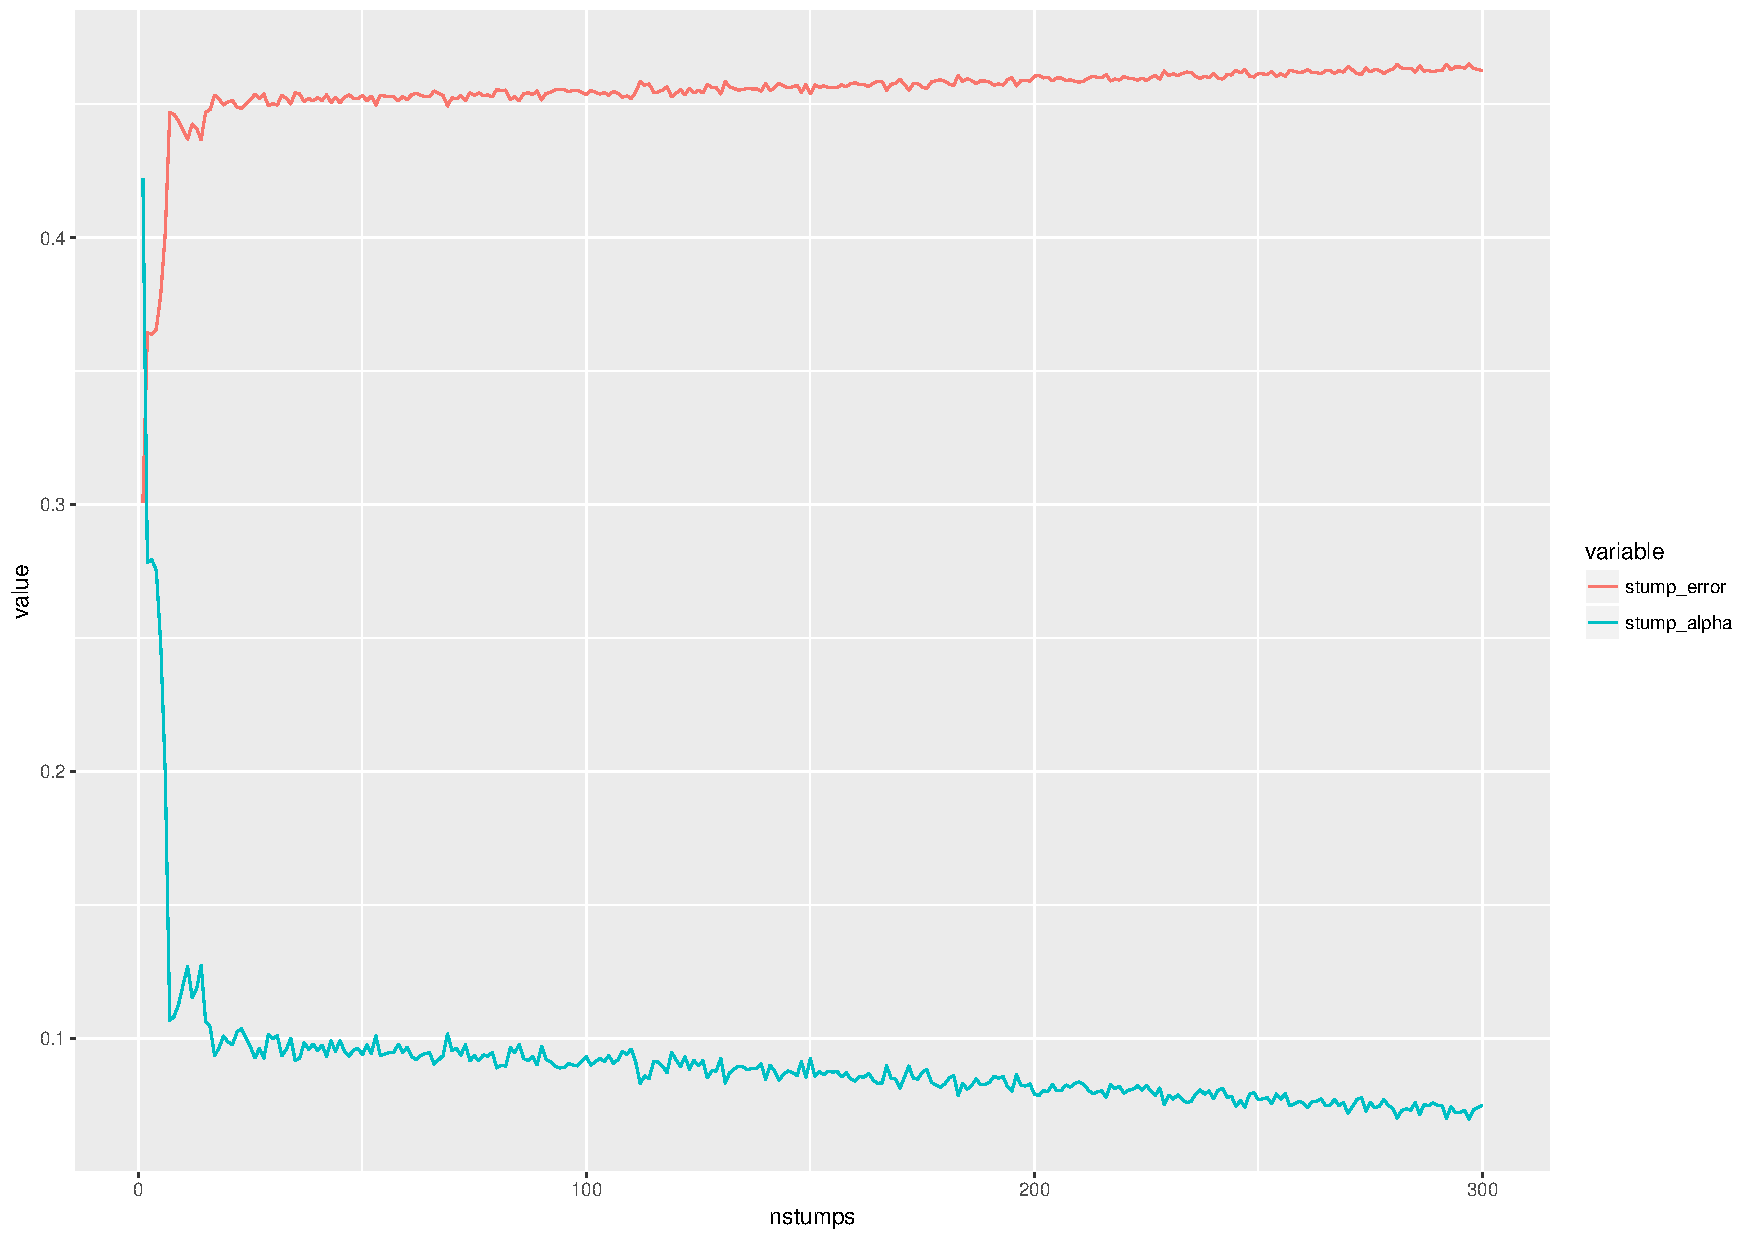
\includegraphics[width=\linewidth]{imgs/alpha_error.pdf}
  \caption{Adaboost \emph{stumps} escolhidos em cada iteração com seus  alphas e errors  associados}
  \label{fig:adaboost_alphas}
\end{figure}

Outra análise interessante é relação dos alphas e dos errors de cada stump escolhido (Pseudocódigo.~\ref{pseudocode:adaboost}, calculo $\alpha_m$), por definição matemática o alpha  e erro do stump estão inversamente relacionados: quem erra mais tem um alpha menor e consecutivamente contribui menos para a classificação final. Como podemos ver pela Figura.~\ref{fig:adaboost_alphas}, os primeiros stumps tendem a ser escolhidos com uma importância (alpha) mais alta e subsecutivamente essas importâncias tendem a decrescer suavemente fazendo com que a importância dos últimos stumps escolhidos sejam aproximadamente iguais. Porem como o \emph{Adaboost} atualiza os pesos de forma que o próximo stump é enviesado para escolher aquele que acerta mais os que o anterior errou, na \emph{big-picture}, mesmo tendo importância próxima eles tendem a contribuir com pouca interseção, são especialistas em partes diferentes dos dados.
